\section{Double Riemann Sums and Double Integrals over Rectangles} \label{S:11.1.Double_Integrals_Rectangles}

\vspace*{-14 pt}
\framebox{\hspace*{3 pt}
\parbox{6.25 in}{\begin{goals}
\item What is a double Riemann sum?
\item How is the double integral of a continuous function $f = f(x,y)$ defined?
\item What are two things the double integral of a function can tell us?
\end{goals}} \hspace*{3 pt}}


\subsection*{Introduction}

In single-variable calculus, recall that we approximated the area under the graph of a positive function $f$ on an interval $[a,b]$ by adding areas of rectangles whose heights are determined by the curve. The general process involved subdividing the interval $[a,b]$ into smaller subintervals, constructing rectangles on each of these smaller intervals to approximate the region under the curve on that subinterval, then summing  the areas of these rectangles to approximate the area under the curve. We will extend this process in this section to its three-dimensional analogs, double Riemann sums and double integrals over rectangles.

\begin{pa} \label{PA:11.1} In this activity we introduce the concept of a double Riemann sum. 
    \ba
    \item  Review the concept of the Riemann sum from single-variable calculus. Then, explain how we define the definite integral $\int_a^b f(x) \ dx$ of a continuous function of a single variable $x$ on an interval $[a,b]$. Include a sketch of a continuous function on an interval $[a,b]$ with appropriate labeling in order to illustrate your definition.


    \item In our upcoming study of integral calculus for multivariable functions, we will first extend the idea of the single-variable definite integral to functions of two variables over rectangular domains. To do so, we will need to understand how to partition a rectangle into subrectangles. Let $R$ be rectangular domain $R = \{(x,y) : 0 \leq x \leq 6, 2 \leq y \leq 4\}$ (we can also represent this domain with the notation $[0,6] \times [2,4]$), as pictured in Figure \ref{F:11.1.Domain}. 
    
        \begin{figure}[ht]
\begin{center}
  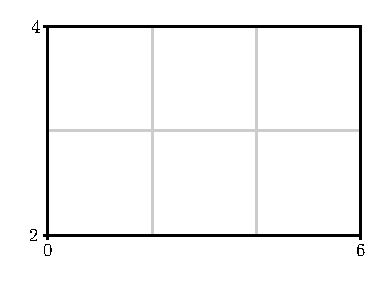
\includegraphics{figures/fig_11_1_rect_domain.eps}
\end{center}
\caption{Rectangular domain $R$ with subrectangles.}
\label{F:11.1.Domain}
\end{figure}
    
To form a partition of the full rectangular region, $R$, we will partition both intervals $[0,6]$ and $[2,4]$; in particular, we choose to partition the interval $[0,6]$ into three uniformly sized subintervals and the interval $[2,4]$ into two evenly sized subintervals as shown in Figure \ref{F:11.1.Domain}. In the following questions, we discuss how to identify the endpoints of each subinterval and the resulting subrectangles.
            \begin{enumerate}[i.]
            \item Let $0=x_0 < x_1 < x_2 < x_3=6$ be the endpoints of the subintervals of $[0,6]$ after partitioning. What is the length $\Delta x$ of each subinterval $[x_{i-1},x_i]$ for $i$ from 1 to 3?
	

    \item Explicitly identify $x_0$, $x_1$, $x_2$, and $x_3$. On Figure \ref{F:11.1.Domain} or your own version of the diagram, label these endpoints.
    	
		
	       \item Let $2=y_0 < y_1 < y_2=4$ be the endpoints of the subintervals of $[2,4]$ after partitioning. What is the length $\Delta y$ of each subinterval $[y_{j-1},y_j]$ for $j$ from 1 to 2? Identify $y_0$, $y_1$, and $y_2$ and label these endpoints on Figure \ref{F:11.1.Domain}.
	

	       \item Let $R_{ij}$ denote the subrectangle $[x_{i-1},x_i] \times [y_{j-1},y_j]$.  Appropriately label each subrectangle in your drawing of Figure \ref{F:11.1.Domain}.  How does the total number of subrectangles depend on the partitions of the intervals $[0,6]$ and $[2,4]$?
	
	
	       \item What is area $\Delta A$ of each subrectangle?

            \end{enumerate}
	\ea
\end{pa}


\begin{activitySolution}
    \ba
    \item  We approximated the area under the graph of a positive function $f$ on an interval $[a,b]$ by adding areas of rectangles. The process was to subdivide the interval $[a,b]$ into smaller subintervals, construct rectangles on each of these smaller intervals to approximate the region under the curve on that subinterval, then use the sum of the areas of these rectangles to approximate the area under the curve.

%\begin{figure}[ht]
%\begin{center}
%\resizebox{!}{2.0in}{\includegraphics{11_1_Riemann_Sum_1}}
%\end{center}
%\caption{A Riemann sum approximating the area under a curve}
%\label{F:11.1.Riemann_Sum_1}
%\end{figure}

In more detail, we started with a continuous function $f$ on a closed interval $[a,b]$. We then partitioned the interval $[a, b]$ into $n$ subintervals of equal length $\Delta x = \frac{b-a}{n}$. Let $x_0$, $x_1$, $\ldots$, $x_n$ be the endpoints of these subintervals, where $a = x_0<x_1<x_2 < \cdots < x_n = b$. We chose a point $x_i^*$ in each subinterval $[x_{i-1},x_i]$ and constructed a rectangle $R_i$ with base the interval  $[x_{i-1},x_i]$ and height $x_i^*$. The area of the rectangle $R_i$ is $f\left(x_i^*\right) \cdot \Delta x$. We then approximate the area under the curve defined by $f$ on the interval $[a,b]$ by the sum
\[\sum_{i=1}^n f\left(x_i^*\right) \cdot \Delta x.\]
%Figure \ref{F:11.1.Riemann_Sum_1} illustrates this process using 15 rectangles to approximate the area under the curve.

If we let $n$ go to infinity, we obtain the exact area under the curve and call this the definite integral of $f$ on the interval $[a,b]$:
\[\int_a^b f(x) \ dx = \lim_{n \to \infty} \sum_{i=1}^n f\left(x_i^*\right) \cdot \Delta x.\]


    \item We determine the endpoints of each subinterval and the resulting subrectangles.
            \begin{enumerate}[i.]
            \item Since these partition points are uniformly spaced, the distance between them is $\Delta x = \frac{6-0}{3} = 2$.

		\item Because $\Delta x = 2$, we have
\[x_0 = 0, \ \ \ x_1 = 2, \ \ \ x_2 = 4, \ \ \ \text{ and } \ \ \ x_3 = 6.\]
These points are labeled in the figure below. %in Figure \ref{F:11.1.Domain_s}.
%\begin{figure}[ht]
\begin{center}
\setlength{\unitlength}{1.0cm}
\begin{picture}(6.5,4.5)
\put(-0.1,-0.3){$x_0$}
\put(1.85,-0.3){$x_1$}
\put(3.85,-0.3){$x_2$}
\put(5.85,-0.3){$x_3$}
\put(-0.45,0.05){$y_0$}
\put(-0.45,1.9){$y_1$}
\put(-0.45,3.9){$y_2$}
\put(0,0){\line(1,0){6}}
\put(0,2){\line(1,0){6}}
\put(0,4){\line(1,0){6}}
\put(0,0){\line(0,1){4}}
\put(2,0){\line(0,1){4}}
\put(4,0){\line(0,1){4}}
\put(6,0){\line(0,1){4}}
\put(0.7,0.9){$R_{11}$}
\put(2.7,0.9){$R_{21}$}
\put(4.7,0.9){$R_{31}$}
\put(0.7,2.9){$R_{12}$}
\put(2.7,2.9){$R_{22}$}
\put(4.7,2.9){$R_{32}$}
\end{picture}
\end{center}
%\caption{Labeled rectangular domain $R$ with subrectangles.}
%\label{F:11.1.Domain_s}
%\end{figure}
		
	       \item Here we have $\Delta y = \frac{4-2}{2} = 1$, and so
\[y_0 = 2, \ \ \ y_1 = 3, \ \ \ \text{ and } \ \ \ y_2 = 4.\]
These points are labeled in Figure \ref{F:11.1.Domain_s}.
	
	       \item If we partition the interval $[0,6]$ into $m$ subintervals and the interval $[2,4]$ into $n$ subintervals, that will partition the rectangle $R$ into $mn$ subintervals. The subrectangles $R_{ij}$ for our particular partition are labeled in Figure \ref{F:11.1.Domain_s}.

	
	       \item The area of a rectangle is length times width, so $\Delta A = \Delta x \ \Delta y$.


            \end{enumerate}
	\ea

\end{activitySolution}

 \afterpa 

\subsection*{Double Riemann Sums over Rectangles}

For the definite integral in single-variable calculus, we considered a continuous function over a closed, bounded interval $[a,b]$.  In multivariable calculus, we will eventually develop the idea of a definite integral over a closed, bounded region (such as the interior of a circle).  We begin with a simpler situation by thinking only about rectangular domains, and will address more complicated domains in the following section.

Let $f = f(x,y)$ be a continuous function defined on a rectangular domain $R = \{(x,y) : a \leq x \leq b, c \leq y \leq d\}$.  As we saw in Preview Activity~\ref{PA:11.1}, the domain is a rectangle $R$ and we want to partition $R$ into subrectangles.  We do this by partitioning each of the intervals $[a,b]$ and $[c,d]$ into subintervals and using those subintervals to create a partition of $R$ into subrectangles.  In the first activity, we address the quantities and notations we will use in order to define double Riemann sums and double integrals.

\begin{activity} \label{A:11.1.1} Let $f(x,y) = 100 - x^2-y^2$ be defined on the rectangular domain $R = [a,b] \times [c,d]$. Partition the interval $[a,b]$ into four uniformly sized subintervals and the interval $[c,d]$ into three evenly sized subintervals as shown in Figure \ref{F:11.1.Domain2}. As we did in Preview Activity \ref{PA:11.1}, we will need a method for identifying the endpoints of each subinterval and the resulting subrectangles.

\begin{figure}[ht]
\begin{center}
  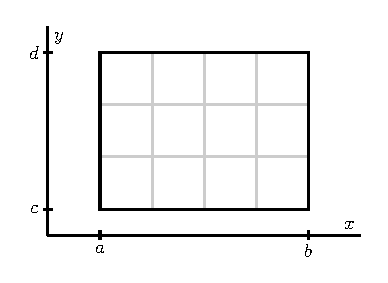
\includegraphics{figures/fig_11_1_rect_general.eps}
\end{center}
\caption{Rectangular domain with subrectangles.}
\label{F:11.1.Domain2}
\end{figure}
 


	\ba
	\item Let $a=x_0 < x_1 < x_2 < x_3 < x_4 =b$ be the endpoints of the subintervals of $[a,b]$ after partitioning. Label these endpoints in Figure \ref{F:11.1.Domain2}.
	
	
	
	\item What is the length $\Delta x$ of each subinterval $[x_{i-1},x_i]$? Your answer should be in terms of $a$ and $b$.
	
	
		
	\item Let $c=y_0 < y_1 < y_2 < y_3 =d$ be the endpoints of the subintervals of $[c,d]$ after partitioning. Label these endpoints in Figure \ref{F:11.1.Domain2}.
	
		
	
	\item What is the length $\Delta y$ of each subinterval $[y_{j-1},y_j]$? Your answer should be in terms of $c$ and $d$.
	
	

	\item The partitions of the intervals $[a,b]$ and $[c,d]$ partition the rectangle $R$ into subrectangles. How many subrectangles are there?
	
	
	
	\item Let $R_{ij}$ denote the subrectangle $[x_{i-1},x_i] \times [y_{j-1},y_j]$. Label each subrectangle in Figure \ref{F:11.1.Domain2}.
	
	
	
	\item What is area $\Delta A$ of each subrectangle?
	
	
	
	\item Now let $[a,b] = [0,8]$ and $[c,d] = [2,6]$.  Let $(x_{11}^*,y_{11}^*)$ be the point in the upper right corner of the subrectangle $R_{11}$. Identify and correctly label this point in Figure \ref{F:11.1.Domain2}. Calculate the product
\[f(x_{11}^*,y_{11}^*) \Delta A.\]
Explain, geometrically, what this product represents.

	
	
	\item For each $i$ and $j$, choose a point $(x_{ij}^*,y_{ij}^*)$ in the subrectangle $R_{i,j}$. Identify and correctly label these points in Figure \ref{F:11.1.Domain2}. Explain what the product
\[f(x_{ij}^*,y_{ij}^*) \Delta A\]
represents.

	
	
	\item \label{p:11.1.Rsum_1} If we were to add all the values $f(x_{ij}^*,y_{ij}^*) \Delta A$ for each $i$ and $j$, what does the resulting number approximate about the surface defined by $f$ on the domain $R$? (You don't actually need to add these values.)

	
	
	\item Write a double sum using summation notation that expresses the arbitrary sum from part ($j$).
	


    \ea


\end{activity}
\begin{smallhint}

\end{smallhint}
\begin{bighint}

\end{bighint}
\begin{activitySolution}
\ba
\item The points $x_0$, $x_1$, $x_2$, $x_3$, and $x_4$ are labeled in the picture below. 
\begin{center}
\setlength{\unitlength}{0.75cm}
\begin{picture}(8.5,6.5)
\put(-0.5,-0.4){$x_0$}
\put(1.7,-0.4){$x_1$}
\put(3.7,-0.4){$x_2$}
\put(5.7,-0.4){$x_3$}
\put(7.7,-0.4){$x_4$}
\put(-1.4,0.05){$y=c$}
%\put(-1.0,1.9){$j=1$}
\put(-1.4,5.9){$y=d$}
\put(0,0){\line(1,0){8}}
\put(0,2){\line(1,0){8}}
\put(0,4){\line(1,0){8}}
\put(0,6){\line(1,0){8}}
\put(0,0){\line(0,1){6}}
\put(2,0){\line(0,1){6}}
\put(4,0){\line(0,1){6}}
\put(6,0){\line(0,1){6}}
\put(8,0){\line(0,1){6}}
\end{picture}
\end{center}

\item The length of the interval $[a,b]$ is $b-a$, and we are dividing the interval into 4 subintervals of equal length. So the length of each subinterval is $\Delta x = \frac{b-a}{4}$. 

\item The points $y_0$, $y_1$, $y_2$, and $y_3$ are labeled in the picture below. 
\begin{center}
\setlength{\unitlength}{0.75cm}
\begin{picture}(8.5,6.5)
\put(-0.5,-0.4){$x_0$}
\put(1.7,-0.4){$x_1$}
\put(3.7,-0.4){$x_2$}
\put(5.7,-0.4){$x_3$}
\put(7.7,-0.4){$x_4$}
\put(-0.7,0){$y_0$}
\put(-0.7,1.9){$y_1$}
\put(-0.7,3.9){$y_2$}
\put(-0.7,5.9){$y_3$}
\put(0,0){\line(1,0){8}}
\put(0,2){\line(1,0){8}}
\put(0,4){\line(1,0){8}}
\put(0,6){\line(1,0){8}}
\put(0,0){\line(0,1){6}}
\put(2,0){\line(0,1){6}}
\put(4,0){\line(0,1){6}}
\put(6,0){\line(0,1){6}}
\put(8,0){\line(0,1){6}}
\end{picture}
\end{center}

\item The length of the interval $[c,d]$ is $d-c$, and we are dividing the interval into 3 subintervals of equal length. So the length of each subinterval is $\Delta y = \frac{d-c}{3}$. 

\item We have 4 subintervals in the $x$ direction and 3 in the $y$ direction, partitioning the rectangle $[a,b] \times [c,d]$ into $3 \times 4 = 12$ subrectangles. 
	
\item As examples, the subrectangle $[x_0,x_1] \times y_0, y_1]$ is $R_{11}$, the lower left subrectangle and the subrectangle $[x_1,x_2] \times y_0, y_1]$ is $R_{21}$, the subrectangle to the right of subrectangle $R_{11}$. The 12 subrectangles are labeled in the figure below.

\begin{center}
\setlength{\unitlength}{0.75cm}
\begin{picture}(8.5,6.5)
\put(-0.5,-0.4){$x_0$}
\put(1.7,-0.4){$x_1$}
\put(3.7,-0.4){$x_2$}
\put(5.7,-0.4){$x_3$}
\put(7.7,-0.4){$x_4$}
\put(-0.7,0){$y_0$}
\put(-0.7,1.9){$y_1$}
\put(-0.7,3.9){$y_2$}
\put(-0.7,5.9){$y_3$}
\put(0.6,0.8){$R_{11}$}
\put(2.6,0.8){$R_{21}$}
\put(4.6,0.8){$R_{31}$}
\put(6.6,0.8){$R_{41}$}
\put(0.6,2.8){$R_{12}$}
\put(2.6,2.8){$R_{22}$}
\put(4.6,2.8){$R_{32}$}
\put(6.6,2.8){$R_{42}$}
\put(6.6,0.8){$R_{41}$}
\put(0.6,4.8){$R_{13}$}
\put(2.6,4.8){$R_{23}$}
\put(4.6,4.8){$R_{33}$}
\put(6.6,4.8){$R_{43}$}
\put(0,0){\line(1,0){8}}
\put(0,2){\line(1,0){8}}
\put(0,4){\line(1,0){8}}
\put(0,6){\line(1,0){8}}
\put(0,0){\line(0,1){6}}
\put(2,0){\line(0,1){6}}
\put(4,0){\line(0,1){6}}
\put(6,0){\line(0,1){6}}
\put(8,0){\line(0,1){6}}
\end{picture}
\end{center}
	
\item Since each subrectangle has side lengths $\frac{b-a}{4}$ and $\frac{d-c}{3}$, the area $\Delta A$ of each subrectangle is $\Delta A = \left(\frac{b-a}{4}\right) \left(\frac{d-c}{3}\right)$. 
	
	
\item With $[a,b] = [0,8]$ and $[c,d] = [2,6]$, we have $\Delta x = 2$ and $\Delta y = \frac{4}{3}$. So $(x_{11}^*,y_{11}^*) 0 \left(2, \frac{4}{3}\right)$ as shown in the figure below. Then
\[f(x_{11}^*,y_{11}^*) \Delta A = f\left(2, \frac{4}{3}\right) (2)\left(\frac{4}{3}\right) = \left(\frac{848}{9}\right)\frac{8}{3} = \frac{6784}{27} \approx 251.26.\]
This result represents the volume of a box with height $f(x_{11}^*,y_{11}^*)$ and base given be the rectangle $[x_0, x_1] \times [y_0, y_1]$. 

\begin{center}
\setlength{\unitlength}{0.75cm}
\begin{picture}(8.5,6.5)
\put(-0.5,-0.4){$x_0$}
\put(1.7,-0.4){$x_1$}
\put(3.7,-0.4){$x_2$}
\put(5.7,-0.4){$x_3$}
\put(7.7,-0.4){$x_4$}
\put(-0.7,0){$y_0$}
\put(-0.7,1.9){$y_1$}
\put(-0.7,3.9){$y_2$}
\put(-0.7,5.9){$y_3$}
\put(0.6,0.8){$R_{11}$}
\put(2.6,0.8){$R_{21}$}
\put(4.6,0.8){$R_{31}$}
\put(6.6,0.8){$R_{41}$}
\put(0.6,2.8){$R_{12}$}
\put(2.6,2.8){$R_{22}$}
\put(4.6,2.8){$R_{32}$}
\put(6.6,2.8){$R_{42}$}
\put(6.6,0.8){$R_{41}$}
\put(0.6,4.8){$R_{13}$}
\put(2.6,4.8){$R_{23}$}
\put(4.6,4.8){$R_{33}$}
\put(6.6,4.8){$R_{43}$}
\put(2,2){\circle*{0.15}}
\put(2.05,2.15){\scriptsize{$(x_{11}^*,y_{11}^*)$}}
\put(0,0){\line(1,0){8}}
\put(0,2){\line(1,0){8}}
\put(0,4){\line(1,0){8}}
\put(0,6){\line(1,0){8}}
\put(0,0){\line(0,1){6}}
\put(2,0){\line(0,1){6}}
\put(4,0){\line(0,1){6}}
\put(6,0){\line(0,1){6}}
\put(8,0){\line(0,1){6}}
\end{picture}
\end{center}
	
	
	\item For each $i$ and $j$, let $(x_{ij}^*,y_{ij}^*)$ be the upper right corner of the subrectangle $R_{i,j}$. These points are marked and labeled in the figure below. 
Identify and correctly label these points in Figure \ref{F:11.1.Domain2}. Explain what the product
\[f(x_{ij}^*,y_{ij}^*) \Delta A\]
represents.

\begin{center}
\setlength{\unitlength}{0.75cm}
\begin{picture}(8.5,6.5)
\put(-0.5,-0.4){$x_0$}
\put(1.7,-0.4){$x_1$}
\put(3.7,-0.4){$x_2$}
\put(5.7,-0.4){$x_3$}
\put(7.7,-0.4){$x_4$}
\put(-0.7,0){$y_0$}
\put(-0.7,1.9){$y_1$}
\put(-0.7,3.9){$y_2$}
\put(-0.7,5.9){$y_3$}
\put(0.6,0.8){$R_{11}$}
\put(2.6,0.8){$R_{21}$}
\put(4.6,0.8){$R_{31}$}
\put(6.6,0.8){$R_{41}$}
\put(0.6,2.8){$R_{12}$}
\put(2.6,2.8){$R_{22}$}
\put(4.6,2.8){$R_{32}$}
\put(6.6,2.8){$R_{42}$}
\put(6.6,0.8){$R_{41}$}
\put(0.6,4.8){$R_{13}$}
\put(2.6,4.8){$R_{23}$}
\put(4.6,4.8){$R_{33}$}
\put(6.6,4.8){$R_{43}$}
\put(2,2){\circle*{0.15}}
\put(2,4){\circle*{0.15}}
\put(2,6){\circle*{0.15}}
\put(4,2){\circle*{0.15}}
\put(4,4){\circle*{0.15}}
\put(4,6){\circle*{0.15}}
\put(6,2){\circle*{0.15}}
\put(6,4){\circle*{0.15}}
\put(6,6){\circle*{0.15}}
\put(8,2){\circle*{0.15}}
\put(8,4){\circle*{0.15}}
\put(8,6){\circle*{0.15}}
\put(2.05,2.15){\scriptsize{$(x_{11}^*,y_{11}^*)$}}
\put(2.05,4.15){\scriptsize{$(x_{12}^*,y_{12}^*)$}}
\put(2.05,6.15){\scriptsize{$(x_{13}^*,y_{13}^*)$}}
\put(4.05,2.15){\scriptsize{$(x_{21}^*,y_{21}^*)$}}
\put(4.05,4.15){\scriptsize{$(x_{22}^*,y_{22}^*)$}}
\put(4.05,6.15){\scriptsize{$(x_{23}^*,y_{23}^*)$}}
\put(6.05,2.15){\scriptsize{$(x_{31}^*,y_{31}^*)$}}
\put(6.05,4.15){\scriptsize{$(x_{32}^*,y_{32}^*)$}}
\put(6.05,6.15){\scriptsize{$(x_{33}^*,y_{33}^*)$}}
\put(8.05,2.15){\scriptsize{$(x_{41}^*,y_{41}^*)$}}
\put(8.05,4.15){\scriptsize{$(x_{42}^*,y_{42}^*)$}}
\put(8.05,6.15){\scriptsize{$(x_{43}^*,y_{43}^*)$}}
\put(0,0){\line(1,0){8}}
\put(0,2){\line(1,0){8}}
\put(0,4){\line(1,0){8}}
\put(0,6){\line(1,0){8}}
\put(0,0){\line(0,1){6}}
\put(2,0){\line(0,1){6}}
\put(4,0){\line(0,1){6}}
\put(6,0){\line(0,1){6}}
\put(8,0){\line(0,1){6}}
\end{picture}
\end{center}
	
	
\item If we add all the values $f(x_{ij}^*,y_{ij}^*) \Delta A$ for each $i$ and $j$, the resulting number approximates the volume of the solid bounded above by the surface defined by $f$ and below by the rectangle $R$. 

	
	
\item A double sum that expresses the arbitrary sum from part ($j$) is
\[\sum_{j=1}^3 \sum_{i=1}^4 f(x_{ij}^*,y_{ij}^*) \Delta A.\]
	


\ea

\end{activitySolution}
\aftera



\subsection*{Double Riemann Sums and Double Integrals}

Now we use the process from the most recent activity to formally define double Riemann sums and double integrals.

\vspace*{5pt}
\nin \framebox{\hspace*{3 pt}
\parbox{6.25 in}{\begin{definition} Let $f$ be a continuous function on a rectangle $R = \{(x,y) : a \leq x \leq b, c \leq y \leq d\}$. A \textbf{double Riemann sum for $f$ over $R$}\index{double Riemann sum} is created as follows.
\begin{itemize}
\item Partition the interval $[a, b]$ into $m$ subintervals of equal length $\Delta x = \frac{b-a}{m}$. Let $x_0$, $x_1$, $\ldots$, $x_m$ be the endpoints of these subintervals, where $a = x_0<x_1<x_2 < \cdots < x_m = b$.
\item Partition the interval $[c, d]$ into $n$ subintervals of equal length $\Delta y = \frac{d-c}{n}$. Let $y_0$, $y_1$, $\ldots$, $y_n$ be the endpoints of these subintervals, where $c = y_0<y_1<y_2 < \cdots < y_n = d$.
\item These two partitions create a partition of the rectangle $R$ into $mn$ subrectangles $R_{ij}$ with opposite vertices $(x_{i-1},y_{j-1})$ and $(x_i, y_j)$ for $i$ between $1$ and $m$ and $j$ between $1$ and $n$. These rectangles all have equal area $\Delta A = \Delta x \cdot \Delta y$.
\item Choose a point $(x_{ij}^*, y_{ij}^*)$ in each rectangle $R_{ij}$. Then, a double Riemann sum for $f$ over $R$ is given by
\[\sum_{j=1}^n \sum_{i=1}^m f(x_{ij}^*, y_{ij}^*) \cdot \Delta A.\]
\end{itemize}
\end{definition}
} \hspace*{3 pt}}
\vspace*{5pt}

If $f(x,y) \geq 0$ on the rectangle $R$, we may ask to find the volume 
of the solid bounded above by $f$ over
$R$, as illustrated on the left of Figure \ref{F:11.1.volume}.  
This volume is approximated by a
Riemann sum, which sums the volumes of the rectangular
boxes shown on the right of Figure \ref{F:11.1.volume}.  

\begin{figure}[ht]
  \begin{center}
    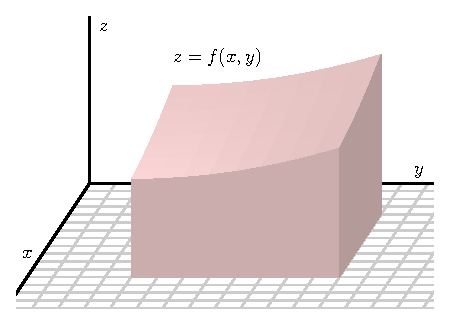
\includegraphics{figures/fig_11_1_volume.eps}
    \hspace*{20pt}
    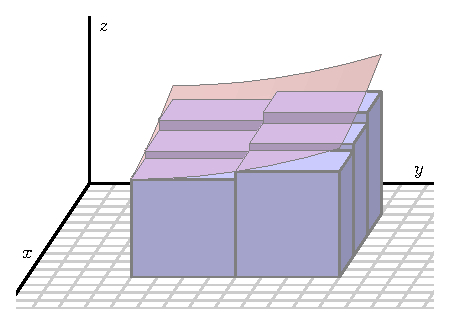
\includegraphics{figures/fig_11_1_riemann_3_2.eps}
  \end{center}
  \caption{The volume under a graph approximated by a Riemann Sum}
  \label{F:11.1.volume}
\end{figure}

As we let the number of
subrectangles increase without bound (in other words, as both $m$ and
$n$ in a double Riemann sum go to infinity), as illustrated in
Figure \ref{F:11.1.rs}, the sum of the volumes of the rectangular boxes
approaches the volume of the solid bounded above by $f$ over
$R$. The value of this limit, provided it exists, is the double integral.

\begin{figure}[ht]
  \begin{center}
    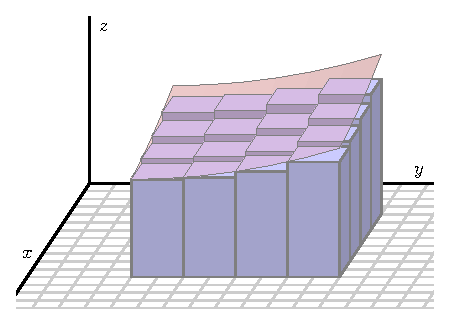
\includegraphics{figures/fig_11_1_riemann_4_4.eps}
    \hspace*{20pt}
    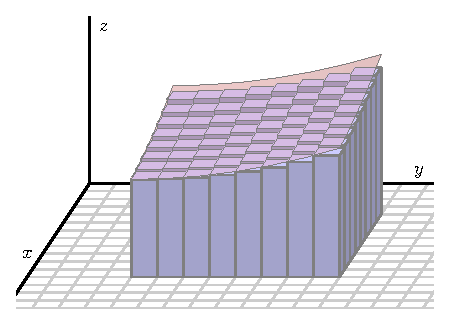
\includegraphics{figures/fig_11_1_riemann_8_8.eps}
  \end{center}
  \caption{Finding better approximations by using smaller subrectangles.}
  \label{F:11.1.rs}
\end{figure}

\vspace*{5pt}
\nin \framebox{\hspace*{3 pt}
\parbox{6.25 in}{ \begin{definition}  Let $R$ be a rectangular region in the $x$-$y$ plane and $f$ a continuous function over $R$. With terms defined as in a double Riemann sum, the \textbf{double integral of $f$ over $R$}\index{double integral!definition} is
\[\iint_R f(x,y) \, dA = \lim_{m,n \to \infty} \sum_{j=1}^n \sum_{i=1}^m f(x_{ij}^*, y_{ij}^*) \cdot \Delta A.\]
\end{definition}
} \hspace*{3 pt}}
\vspace*{5pt}


\subsection*{Interpretation of Double Riemann Sums and Double integrals.}

At the moment, there are two ways we can interpret the value of the double integral.

\begin{itemize}
\item Suppose that $f(x,y)$ assumes both positive and negatives
  values on the rectangle $R$, as shown on the left of Figure
  \ref{F:11.1.signed}.  When constructing a Riemann sum, for each $i$ and $j$, the product $f(x_{ij}^*, y_{ij}^*) \cdot \Delta A$
can be interpreted as a ``signed" volume of a box with base area $\Delta A$ and ``signed" height $f(x_{ij}^*, y_{ij}^*)$. Since $f$ can have negative values, this ``height" could be negative. The sum
\[\sum_{j=1}^n \sum_{i=1}^m f(x_{ij}^*, y_{ij}^*) \cdot \Delta A\]
can then be interpreted as a sum of ``signed" volumes of boxes, with a
negative sign attached to those boxes whose heights are below the
$xy$-plane. 
\begin{figure}[ht]
  \begin{center}
    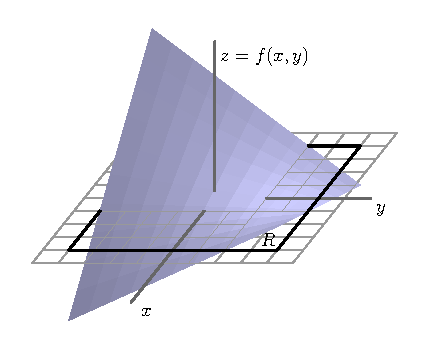
\includegraphics{figures/fig_11_1_signed_graph.eps}
    \hspace*{20pt}
    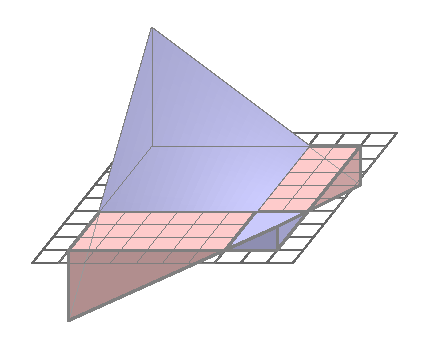
\includegraphics{figures/fig_11_1_signed_volume.eps}
  \end{center}
  \caption{The integral measures signed volume.}
  \label{F:11.1.signed}
\end{figure}
We can then realize the double integral $\iint_R
f(x,y) \, dA$ as a difference in volumes\index{double
  integral!difference in volumes}: $\iint_R f(x,y) \, dA$ tells us
the volume of the solids the graph of $f$ bounds above the $xy$-plane
over the rectangle $R$ minus the volume of the solids the graph of $f$
bounds below the $xy$-plane under the rectangle $R$.  This is shown on
the right of Figure \ref{F:11.1.signed}.



\item The average of the finitely many $mn$ values $f(x_{ij}^*, y_{ij}^*)$ that we take in a double Riemann sum is given by
\[\mbox{Avg}_{mn} = \frac{1}{mn} \sum_{j=1}^n \sum_{i=1}^m f(x_{ij}^*, y_{ij}^*).\]
If we take the limit as $m$ and $n$ go to infinity, we obtain what we define as the average value\index{double integral!average value} of $f$ over the region $R$, which is connected to the value of the double integral. First, to view $\text{Avg}_{mn}$ as a double Riemann sum, note that
\[\Delta x = \frac{b-a}{m} \ \ \ \ \ \text{ and } \ \ \ \ \ \Delta y = \frac{d-c}{n}.\]
Thus,
\[\frac{1}{mn} = \frac{\Delta x \cdot \Delta y}{(b-a)(d-c)} = \frac{\Delta A}{A(R)},\]
where $A(R)$ denotes the area of the rectangle $R$. Then, the average value of the function $f$ over $R$, $f_{\mbox{\tiny{AVG}(R)}}$, is given by
\begin{align*}
f_{\mbox{\tiny{AVG}(R)}} & = \lim_{m,n \to \infty} \frac{1}{mn} \sum_{j=1}^n \sum_{i=1}^m f(x_{ij}^*, y_{ij}^*) \\
				    & = \lim_{m,n \to \infty} \frac{1}{A(R)} \sum_{j=1}^n \sum_{i=1}^m f(x_{ij}^*, y_{ij}^*) \cdot \Delta A \\
				    & = \frac{1}{A(R)} \iint_R f(x,y) \, dA.
\end{align*}
Therefore, the double integral of $f$ over $R$ divided by the area of $R$ gives us the average value of the function $f$ on $R$. Finally, if $f(x, y) \geq  0$ on $R$, we can interpret this average value of $f$ on $R$ as the height of the box with base $R$ that has the same volume as the volume of the surface defined by $f$ over $R$.
\end{itemize}

\begin{activity} \label{A:11.1.2} Let $f(x,y) = x+2y$ and let $R = [0,2] \times [1,3]$.
	\ba
	\item Draw a picture of $R$. Partition $[0,2]$ into 2 subintervals of equal length and the interval $[1,3]$ into two subintervals of equal length. Draw these partitions on your picture of $R$ and label the resulting subrectangles using the labeling scheme we established in the definition of a double Riemann sum.
	
	
	
	\item For each $i$ and $j$, let $(x_{ij}^*, y_{ij}^*)$ be the midpoint of the rectangle $R_{ij}$. Identify the coordinates of each $(x_{ij}^*, y_{ij}^*)$. Draw these points on your picture of $R$.
	
	
	
	\item Calculate the Riemann sum
\[\sum_{j=1}^n \sum_{i=1}^m f(x_{ij}^*, y_{ij}^*) \cdot \Delta A\]
using the partitions we have described. If we let $(x_{ij}^*, y_{ij}^*)$ be the midpoint of the rectangle $R_{ij}$ for each $i$ and $j$, then the resulting Riemann sum is called a \emph{midpoint sum}.



	\item Give two interpretations for the meaning of the sum you just calculated.


    \ea


\end{activity}
\begin{smallhint}

\end{smallhint}
\begin{bighint}

\end{bighint}
\begin{activitySolution}
	\ba
	\item The partition of $[0,2]$ into 2 subintervals of equal length yields endpoints $0$, $1$ and $2$, while the partition of the interval $[1,3]$ into two subintervals of equal length produces endpoints $1$, $2$, and $3$. The partitions of the intervals divide the rectangle $R$ into $4$ subrectangles of area 1 as shown in the figure below. 
\begin{center}
\setlength{\unitlength}{0.75cm}
\begin{picture}(4.5,6.5)
\put(-0.1,-0.6){$0$}
\put(1.9,-0.6){$1$}
\put(3.9,-0.6){$2$}
\put(-0.4,1.85){$1$}
\put(-0.4,3.85){$2$}
\put(-0.4,5.85){$3$}
\put(0.6,2.8){$R_{11}$}
\put(2.6,2.8){$R_{21}$}
\put(0.6,4.8){$R_{12}$}
\put(2.6,4.8){$R_{22}$}
%Horizontal lines
\put(0,0){\line(1,0){5}}
\put(-0.1,2){\line(1,0){4.1}}
\put(-0.1,4){\line(1,0){4.1}}
\put(-0.1,6){\line(1,0){4.1}}
\put(4.9,-0.6){$x$}
%Vertical lines
\put(0,0){\line(0,1){7}}
\put(2,2){\line(0,1){4}}
\put(4,2){\line(0,1){4}}
\put(-0.4,6.9){$y$}
%Vertical tick marks
\put(2,-0.1){\line(0,1){0.2}}
\put(4,-0.1){\line(0,1){0.2}}

\end{picture}
\end{center}
		
	
	
	\item The point $(x_{11}^*, y_{11}^*)$ is the midpoint of the rectangle $[0,1] \times [1,2]$, and so $(x_{11}^*, y_{11}^*) = (0.5, 1.5)$. Similarly, we have $(x_{21}^*, y_{21}^*) = (1.5, 1.5)$, $(x_{12}^*, y_{12}^*) = (0.5, 2.5)$, and $(x_{22}^*, y_{22}^*) = (1.5, 2.5)$. These points are shown in the figure below. 
\begin{center}
\setlength{\unitlength}{0.75cm}
\begin{picture}(4.5,6.5)
\put(-0.1,-0.6){$0$}
\put(1.9,-0.6){$1$}
\put(3.9,-0.6){$2$}
\put(-0.4,1.85){$1$}
\put(-0.4,3.85){$2$}
\put(-0.4,5.85){$3$}
%\put(0.6,2.8){$R_{11}$}
%\put(2.6,2.8){$R_{21}$}
%\put(0.6,4.8){$R_{12}$}
%\put(2.6,4.8){$R_{22}$}
\put(1,3){\circle*{0.1}}
\put(1,5){\circle*{0.1}}
\put(3,3){\circle*{0.1}}
\put(3,5){\circle*{0.1}}
\put(0.2,2.5){\scriptsize{$(x_{11}^*,y_{11}^*)$}}
\put(0.2,4.5){\scriptsize{$(x_{12}^*,y_{12}^*)$}}
\put(2.2,2.5){\scriptsize{$(x_{21}^*,y_{21}^*)$}}
\put(2.2,4.5){\scriptsize{$(x_{22}^*,y_{22}^*)$}}
%Horizontal lines
\put(0,0){\line(1,0){5}}
\put(-0.1,2){\line(1,0){4.1}}
\put(-0.1,4){\line(1,0){4.1}}
\put(-0.1,6){\line(1,0){4.1}}
\put(4.9,-0.6){$x$}
%Vertical lines
\put(0,0){\line(0,1){7}}
\put(2,2){\line(0,1){4}}
\put(4,2){\line(0,1){4}}
\put(-0.4,6.9){$y$}
%Vertical tick marks
\put(2,-0.1){\line(0,1){0.2}}
\put(4,-0.1){\line(0,1){0.2}}

\end{picture}
\end{center}
		
	
	
	\item Writing out the terms and calculating yields
\begin{align*}
\sum_{j=1}^n \sum_{i=1}^m f(x_{ij}^*, y_{ij}^*) \cdot \Delta A &= f(0.5, 1.5)(1) + f(1.5, 1.5)(1) + f(0.5, 2.5)(1) + f(1.5, 2.5)(1) \\
	&= 3.5+4.5+5.5+6.5 \\
	&= 20.
\end{align*}


	\item Since $f(x,y) \geq 0$ on $R$, the sum in part (b) approximates the volume of the solid bounded above by the graph of $f$ and below by the rectangle $R$. In addition, the sum also approximates the average value of $f$ on $R$ times the area of $R$. 


    \ea
\end{activitySolution}
\aftera



\begin{activity} \label{A:11.1.3} Let $f(x,y) = \sqrt{4-y^2}$ on the rectangular domain $R = [1,7] \times [-2,2]$. Partition $[1,7]$ into 3 equal length subintervals and $[-2,2]$ into 2 equal length subintervals. A table of values of $f$ at some points in $R$ is given in Table \ref{DI:11.1.TOV}, and a graph of $f$ with the indicated partitions is shown in Figure \ref{F:11.1.DI_example}.

\begin{figure}[ht]
\begin{center}
\begin{minipage}{2.5in}
\begin{center}
\begin{tabular}{|c||c|c|c|c|c|} \hline
    &$-2$   &$-1$       &$0$    &$1$        &$2$ \\ \hhline{|=|=|=|=|=|=|}
$1$ &$0$    &$\sqrt{3}$ &$2$    &$\sqrt{3}$ &$0$ \\ \hline
$2$ &$0$    &$\sqrt{3}$ &$2$    &$\sqrt{3}$ &$0$ \\ \hline
$3$ &$0$    &$\sqrt{3}$ &$2$    &$\sqrt{3}$ &$0$ \\ \hline
$4$ &$0$    &$\sqrt{3}$ &$2$    &$\sqrt{3}$ &$0$ \\ \hline
$5$ &$0$    &$\sqrt{3}$ &$2$    &$\sqrt{3}$ &$0$ \\ \hline
$6$ &$0$    &$\sqrt{3}$ &$2$    &$\sqrt{3}$ &$0$ \\ \hline
$7$ &$0$    &$\sqrt{3}$ &$2$    &$\sqrt{3}$ &$0$ \\ \hline
\end{tabular}
\end{center}
\captionof{table}{Table of values of $f(x,y) =  \sqrt{4-y^2}$.}
\label{DI:11.1.TOV}
\end{minipage} \hspace{0.5in}
\begin{minipage}{2.5in}
\begin{center}
%\resizebox{!}{1.5in}{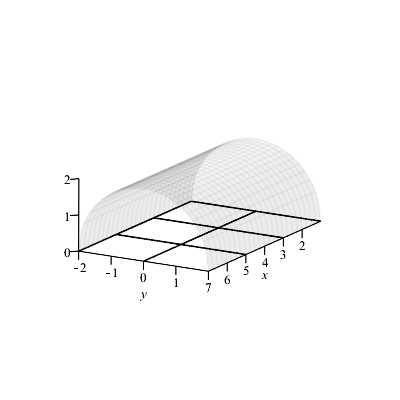
\includegraphics[trim=2cm 3.5cm 2cm 4.5cm, clip]{11_1_DI_example}}
  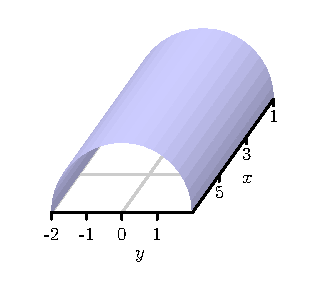
\includegraphics{figures/fig_11_1_cylinder.eps}
%crop graphics in animate trim=<left> <bottom> <right> <top>, add, clip with \includegraphics
\end{center}
\captionof{figure}{Graph of $f(x,y) =  \sqrt{4-y^2}$ on $R$.}
\label{F:11.1.DI_example}
\end{minipage}
\end{center}
\end{figure}

    \ba
    \item Outline the partition of $R$ into subrectangles on the table of values in Table \ref{DI:11.1.TOV}.



    \item Calculate the double Riemann sum using the given partition of $R$ and the values of $f$ in the upper right corner of each subrectangle.


    \item Use geometry to calculate the exact value of $\iint_R f(x,y) \, dA$ and compare it to your approximation. How could we obtain a better approximation?



    \ea

\end{activity}
\begin{smallhint}

\end{smallhint}
\begin{bighint}

\end{bighint}
\begin{activitySolution}
    \ba
    \item The endpoints of the partition of $[1,7]$ are $1$, $3$, $5$, and $7$, while the endpoints of the partition of $[-2,2]$ are $-2$, $0$, and $2$. This makes subrectangles $R_{11} = [1,3] \times [-2,0]$, $R_{21} = [3,5] \times [-2,0]$, $R_{31} = [5,7] \times [-2,0]$, $R_{12} = [1,3] \times [0,2]$, $R_{22} = [3,5] \times [0,2]$, $R_{32} = [5,7] \times [0,2]$. These subrectangles are outlined in the table below.
\begin{center}
\setlength{\unitlength}{0.8cm}
\begin{picture}(6,8)
%Horizontal lines
\put(0,0){\line(1,0){6}}
%\put(0,1){\line(1,0){6}}
%\put(0,2){\line(1,0){6}}
%\put(0,3){\line(1,0){6}}
%\put(0,4){\line(1,0){6}}
%\put(0,5){\line(1,0){6}}
%\put(0,6){\line(1,0){6}}
\put(0,7){\line(1,0){6}}
\put(0,8){\line(1,0){6}}
\put(0,2.5){\line(1,0){6}}
\put(0,4.5){\line(1,0){6}}
%Vertical lines
\put(0,0){\line(0,1){8}}
\put(1,0){\line(0,1){8}}
%\put(2,0){\line(0,1){8}}
%\put(3,0){\line(0,1){8}}
%\put(4,0){\line(0,1){8}}
%\put(5,0){\line(0,1){8}}
\put(6,0){\line(0,1){8}}
\put(3.5,0){\line(0,1){8}}
%Table entries
\put(1.2,7.4){$-2$}
\put(2.2,7.4){$-1$}
\put(3.4,7.4){$0$}
\put(4.4,7.4){$1$}
\put(5.4,7.4){$2$}
\put(0.4,6.4){$1$}
\put(1.4,6.4){$0$}
\put(2.15,6.4){$\sqrt{3}$}
\put(3.4,6.4){$2$}
\put(4.15,6.4){$\sqrt{3}$}
\put(5.4,6.4){$0$}
\put(0.4,5.4){$2$}
\put(1.4,5.4){$0$}
\put(2.15,5.4){$\sqrt{3}$}
\put(3.4,5.4){$2$}
\put(4.15,5.4){$\sqrt{3}$}
\put(5.4,5.4){$0$}
\put(0.4,4.4){$3$}
\put(1.4,4.4){$0$}
\put(2.15,4.4){$\sqrt{3}$}
\put(3.4,4.4){$2$}
\put(4.15,4.4){$\sqrt{3}$}
\put(5.4,4.4){$0$}
\put(0.4,3.4){$4$}
\put(1.4,3.4){$0$}
\put(2.15,3.4){$\sqrt{3}$}
\put(3.4,3.4){$2$}
\put(4.15,3.4){$\sqrt{3}$}
\put(5.4,3.4){$0$}
\put(0.4,2.4){$5$}
\put(1.4,2.4){$0$}
\put(2.15,2.4){$\sqrt{3}$}
\put(3.4,2.4){$2$}
\put(4.15,2.4){$\sqrt{3}$}
\put(5.4,2.4){$0$}
\put(0.4,1.4){$6$}
\put(1.4,1.4){$0$}
\put(2.15,1.4){$\sqrt{3}$}
\put(3.4,1.4){$2$}
\put(4.15,1.4){$\sqrt{3}$}
\put(5.4,1.4){$0$}
\put(0.4,0.4){$7$}
\put(1.4,0.4){$0$}
\put(2.15,0.4){$\sqrt{3}$}
\put(3.4,0.4){$2$}
\put(4.15,0.4){$\sqrt{3}$}
\put(5.4,0.4){$0$}
\end{picture}
\end{center}


    \item Choosing points in the upper right corner of each subrectangle gives us $(x_{11}^*, y_{11}^*) = (3,0)$, $(x_{21}^*, y_{21}^*) = (5,0)$, $(x_{31}^*, y_{31}^*) = (7,0)$, $(x_{12}^*, y_{12}^*) = (3,2)$, $(x_{22}^*, y_{22}^*) = (5,2)$, and $(x_{32}^*, y_{32}^*) = (7,2)$. So 
\begin{align*}
\sum_{j=1}^n \sum_{i=1}^m f\left(x_{ij}^*, y_{ij}^*\right) \cdot \Delta A &= f(3,0)(4) + f(5,0)(4) + f(7,0)(4) + f(3,2)(4) + f(5,3)(4) + f(7,2)(4) \\
	&= 24.
\end{align*}

    \item Since the cross sections parallel to the $yz$-plane are semi-circles of radius 2, we can multiply the area of a cross section by the width to obtain the volume. So the exact volume of this object is $4 \pi (6) = 24 \pi$. We could get a better approximation by using finer partitions.  


    \ea
\end{activitySolution}
\aftera



We conclude this section with a list of properties of double integrals. Since similar properties are satisfied by single-variable integrals and the arguments for double integrals are essentially the same, we omit their justification.

\vspace*{5pt}
\nin \framebox{\hspace*{3 pt}
\parbox{6.25 in}{\textbf{Properties of Double Integrals.} Let $f$ and $g$ be continuous functions on a rectangle $R = \{(x,y) : a \leq x \leq b, c \leq y \leq d\}$, and let $k$ be a constant. Then
\begin{enumerate}
\item $\iint_R (f(x,y) + g(x,y)) \, dA = \iint_R f(x,y) \, dA + \iint_R g(x,y) \, dA$.
\item $\iint_R kf(x,y) \, dA = k \iint_R f(x,y) \, dA$.
\item If $f(x,y) \geq g(x,y)$ on $R$, then $\iint_R f(x,y) \, dA \geq \iint_R g(x,y) \, dA$.
\end{enumerate}
} \hspace*{3 pt}}
\vspace*{5pt}

\begin{summary}
\item Let $f$ be a continuous function on a rectangle $R = \{(x,y) : a \leq x \leq b, c \leq y \leq d\}$. The double Riemann sum for $f$ over $R$ is created as follows.
    \begin{itemize}
    \item[-] Partition the interval $[a, b]$ into $m$ subintervals of equal length $\Delta x = \frac{b-a}{m}$. Let $x_0$, $x_1$, $\ldots$, $x_m$ be the endpoints of these subintervals, where $a = x_0<x_1<x_2 < \cdots < x_m = b$.
    \item[-] Partition the interval $[c, d]$ into $n$ subintervals of equal length $\Delta y = \frac{d-c}{n}$. Let $y_0$, $y_1$, $\ldots$, $y_n$ be the endpoints of these subintervals, where $c = y_0<y_1<y_2 < \cdots < y_n = d$.
    \item[-] These two partitions create a partition of the rectangle $R$ into $mn$ subrectangles $R_{ij}$ with opposite vertices $(x_{i-1},y_{j-1})$ and $(x_i, y_j)$ for $i$ between $1$ and $m$ and $j$ between $1$ and $n$. These rectangles all have equal area $\Delta A = \Delta x \cdot \Delta y$.
    \item[-] Choose a point $(x_{ij}^*, y_{ij}^*)$ in each rectangle $R_{ij}$. Then a double Riemann sum for $f$ over $R$ is given by
    \[\sum_{j=1}^n \sum_{i=1}^m f(x_{ij}^*, y_{ij}^*) \cdot \Delta A.\]
    \end{itemize}
\item With terms defined as in the Double Riemann Sum, the double integral of $f$ over $R$ is
\[\iint_R f(x,y) \, dA = \lim_{m,n \to \infty} \sum_{j=1}^n \sum_{i=1}^m f(x_{ij}^*, y_{ij}^*) \cdot \Delta A.\]
\item Two interpretations of the double integral $\ds \iint_R f(x,y) \, dA$ are:
    \begin{itemize}
    \item[-] The volume of the solids the graph of $f$ bounds above the $xy$-plane over the rectangle $R$ minus the volume of the solids the graph of $f$ bounds below the $xy$-plane under the rectangle $R$;
    \item[-] Dividing the double integral of $f$ over $R$ by the area of $R$ gives us the average value of the function $f$ on $R$. If $f(x, y) \geq  0$ on $R$, we can interpret this average value of $f$ on $R$ as the height of the box with base $R$ that has the same volume as the volume of the surface defined by $f$ over $R$.
    \end{itemize}
\end{summary}


\nin \hrulefill

\begin{exercises} 

\item The temperature at any point on a metal plate in the $xy$ plane is given by $T(x,y) = 100-4x^2 - y^2$, where $x$ and $y$ are measured in inches and $T$ in degrees Celsius.  Consider the portion of the plate that lies on the rectangular region $R = [1,5] \times [3,6]$.

\ba
	\item Estimate the value of $\iint_R T(x,y) \, dA$ by using a double Riemann sum with two subintervals in each direction and choosing $(x_i^*, y_j^*)$ to be the point that lies in the upper right corner of each subrectangle.  
	\item Determine the area of the rectangle $R$.
	\item Estimate the average temperature, $T_{\mbox{\tiny{AVG}(R)}}$, over the region $R$.
	\item Do you think your estimate in (c) is an over- or under-estimate of the true temperature?  Why?
\ea

\begin{exerciseSolution}
\ba
	\item The partition points in the $x$ direction are $1$, $3$, and $5$ and the partition points in the $y$ direction are $3$, $4.5$, and $6$. Using the points that lie in the upper right corner of each subrectangle we have
\[\iint_R T(x,y) \, dA \approx T(3,4.5)(3) + T(5,4.5)(3) + T(3,6)(3) + T(5,6)(3) = 46.5.\]

	\item The area of the rectangle $R$ is $(4)(3) = 12$. 

	\item Using the result of part (a) we approximate the average temperature over $R$ as 
\[T_{\mbox{\tiny{AVG}(R)}} = \frac{1}{\text{Area}(R)} \iint_R T(x,y) \approx \frac{46.5}{12} = 3.875.\]

	\item The temperature function is decreasing in both the $x$ and $y$ directions, so the value at the upper right corner of each subrectangle is the smallest temperature on that subrectangle. So our approximation is an underestimate. 
\ea
\end{exerciseSolution}

\item The wind chill, as frequently   reported, is a measure of how cold it feels outside when the wind is blowing.  In Table \ref{T:11.1.Ex.wind.chill}, the wind chill $w=w(v,T)$, measured in degrees Fahrenheit, is a function of the wind speed $v$, measured in miles per hour, and the ambient air temperature $T$, also measured in degrees Fahrenheit. Approximate the average wind chill on the rectangle $[5,35] \times [-20,20]$ using 3 subintervals in the $v$ direction, 4 subintervals in the $T$ direction, and the point in the lower left corner in each subrectangle. 
\begin{table}[ht] 
  \begin{center}
    \begin{tabular}{|c||c|c|c|c|c|c|c|c|c|}
      \hline
      $v \backslash T$  
         &-20 &-15 &-10 &-5  &0   &5   &10  &15  &20  \\
      \hhline{|=||=|=|=|=|=|=|=|=|=|}
      5  &-34 &-28 &-22 &-16 &-11 &-5 &1 &7 &13  \\
      \hline
      10 &-41 &-35 &-28 &-22 &-16 &-10 &-4 &3 &9   \\
      \hline
      15  &-45 &-39 &-32 &-26 &-19 &-13 &-7 &0 &6  \\
      \hline
      20 &-48 &-42 &-35 &-29 &-22 &-15 &-9 &-2 &4  \\
      \hline
      25 &-51 &-44 &-37 &-31 &-24 &-17 &-11 &-4 &3 \\
      \hline
      30  &-53 &-46 &-39 &-33 &-26 &-19 &-12 &-5 &1 \\
      \hline
      35  &-55 &-48 &-41 &-34 &-27 &-21 &-14 &-7 &0 \\
      \hline
    \end{tabular}
    \caption{Wind chill as a function of wind speed and temperature.}
    \label{T:11.1.Ex.wind.chill}
  \end{center}
\end{table}

\begin{exerciseSolution}
The length of each subinterval in the $v$ direction is $\frac{35-5}{3} = 10$, so our partition points in the $v$ direction are $5$, $15$, $25$, and $35$. The length of each subinterval in the $T$ direction is $\frac{20-(-20)}{4} = 10$, so our partition points in the $T$ direction are $-20$, $-10$, $0$, $10$, and $20$. So
\begin{align*}
\iint w(v,t) \, dA &\approx w(5,-20)(100) + w(15,-20)(100) + w(25,-20)(100) \\
	&\qquad + w(5,-10)(100) + w(15,-10)(100) + w(25,-10)(100) \\
	&\qquad + w(5,0)(100) + w(15,0)(100) + w(25,0)(100)  \\
	&\qquad + w(5,10)(100) + w(15,10)(100) + w(25,10)(100) \\
	&= -29200.
\end{align*}
So the average wind chill on $R$ is approximately
\[ \frac{1}{\text{Area}(R)} \iint_R w(v,T) \approx -\frac{29200}{(30)(40)} = -\frac{73}{3} \approx -24.33.\]
	
\end{exerciseSolution}

\item Consider the box with a sloped top that is given by the following description:  the base is the rectangle $R = [0,4] \times [0,3]$, while the top is given by the plane $z = p(x,y) = 20 - 2x - 3y$.

\ba
	\item Estimate the value of $\iint_R p(x,y) \, dA$ by using a double Riemann sum with four subintervals in the $x$ direction and three subintervals in the $y$ direction, and choosing $(x_i^*, y_j^*)$ to be the point that is the midpoint of each subrectangle.  
	\item What important quantity does your double Riemann sum in (a) estimate?
	\item Suppose it can be determined that $\iint_R p(x,y) \, dA = 138$.  What is the exact average value of $p$ over $R$?
	\item If you wanted to build a rectangular box (with the same base) that has the same volume as the box with the sloped top described here, how tall would the rectangular box have to be?
\ea

\begin{exerciseSolution}
\ba
	\item Our partition points in the $x$ direction are $0$, $1$, $2$, $3$, and $4$ while the partition points in the $y$ direction are $0$, $1$, $2$, and $3$. So 
\begin{align*}
\iint_R p(x,y) \, dA \approx p(0.5,0.5)(1) &+ p(1.5, 0.5)(1) + p(2.5,0.5)(1) + p(3.5,0.5)(1) \\
	&\qquad + p(0.5,1.5)(1) + p(1.5, 1.5)(1) + p(2.5,1.5)(1) + p(3.5,1.5)(1) \\
	&\qquad + p(0.5,2.5)(1) + p(1.5, 2.5)(1) + p(2.5,2.5)(1) + p(3.5,2.5)(1) \\
	&=  138.
\end{align*}

	\item Since $p(x,y) \geq 0$ on $R$, the geometric quantity our double Riemann sum approximates is the volume of the surface with the plane defined by $p$ as the top and with base $R$. 
 
	\item The area of $R$ is 12, so the exact average value of $p$ over $R$ is 
	\[ \frac{1}{\text{Area}(R)} \iint_R p(x,y) \approx \frac{138}{12} = 11.5.\]
	
	\item If $h$ is the height of the box, then we would need to have $12h=138$, or $h = 11.5$. This is the average value of $p$ over $R$. 
\ea
\end{exerciseSolution}



\end{exercises}
\afterexercises


\clearpage
